% Title page
\frame[plain]{\titlepage}

\lecture{Введение}{intro}

\section{Факты, правила и запросы}
\subsection{Основные пункты}

\begin{frame}
	\frametitle{\insertsection}
	\framesubtitle{\insertsubsection}
	\begin{itemize}
		\item Рассмотреть простые примеры программ на \textbf{Prolog}, определить понятия факта, правила, запроса и базы знаний
		\item Дать определения основных понятий и синтаксических конструкций, таких как атомы, переменные и термы
	\end{itemize}
\end{frame}

\subsection{База знаний}

\begin{frame}
	\frametitle{\insertsection}
	\framesubtitle{\insertsubsection}
	Базовые конструкции языка \textbf{Prolog}:
	\begin{itemize}
		\item Факты
		\item Правила
		\item Запросы
	\end{itemize}
	Программа на Prolog представляет собой множество \textbf{фактов} и \textbf{правил}~--- \alert{Базу Знаний}
	Чтобы использовать информацию, содержащуюся в базе знаний, необходимо ставить \textbf{запросы}.
\end{frame}

\begin{frame}
	\frametitle{\insertsection}
	\framesubtitle{\insertsubsection}
	Пример 1
	
	
	\texttt{\begin{itemize}
				\item[] woman(mia).
				\item[] woman(jody).
				\item[] woman(yolanda).
				\item[] playsGuitar(jody).
				\item[]<2-> listensToMusic(mia).
				\item[]<2-> musician(yolanda).
				\item[]<2-> playsGuitar(mia) :- listensToMusic(mia).
				\item[]<2-> playsGuitar(yolanda) :- listensToMusic(yolanda).
				\item[]<2-> listensToMusic(yolanda) :- musician(yolanda).
			\end{itemize}}
\end{frame}

\begin{frame}
	\frametitle{\insertsection}
	\framesubtitle{\insertsubsection}
	Пример 2
	
	
	\texttt{\begin{itemize}
		\item[] musician(mia).
		\item[] listensToMusic(jody).
		\item[] playsGuitar(mia) :- listensToMusic(mia),musician(mia).
		\item[] playsGuitar(jody) :- musician(jody); listensToMusic(jody).
	\end{itemize}}
\end{frame}

\begin{frame}
	\frametitle{\insertsection}
	\framesubtitle{\insertsubsection}
	Пример 3
	
	
	\texttt{\begin{itemize}
		\item[] woman(mia).
		\item[] woman(jody).
		\item[] woman(yolanda).
		\item[] loves(vincent,mia).
		\item[] loves(marcellus,mia).
	\end{itemize}}
\end{frame}

\begin{frame}
	\frametitle{\insertsection}
	\framesubtitle{\insertsubsection}
	Пример 4
	
	
	\texttt{\begin{itemize}
			\item[] loves(vincent,mia).
			\item[] loves(marcellus,mia).
			\item[] jealous(X,Y) :- loves(X,Z),loves(Y,Z).
	\end{itemize}}
\end{frame}

\subsection{Синтаксис}

\begin{frame}
	\frametitle{\insertsection}
	\framesubtitle{\insertsubsection}
	\textbf{\underline{Атомы}}
	
	\begin{enumerate}
		\item Последовательность строчных или прописных букв, цифр и символов подчерка, начинающаяся со строчной буквы.
		\item Произвольная последовательность символов, заключённая в одинарные кавычки.
		\item Последовательность спецсимволов.
	\end{enumerate}

	\begin{rexample}
		mia, marcellus, big\_kahuna\_burger, 'Произвольная строка символов', ====>, :-
	\end{rexample}
\end{frame}

\begin{frame}
	\frametitle{\insertsection}
	\framesubtitle{\insertsubsection}
	\textbf{\underline{Числа}}
	
	\begin{enumerate}
		\item Действительные числа: 2,718; 103,3087; \(\pi \), \ldots
		\item Целые числа: -2, -1, 0, 1, 2, \ldots
	\end{enumerate}

	\textbf{\underline{Переменные}}
	
	\textit{Переменной} называется последовательность строчных или прописных букв, цифр и символов подчерка, начинающаяся с \textbf{прописной буквы} или \textbf{символа подчерка}.
	
	\begin{rexample}
		X, Y, Variable, \_X, X1, \_variable\_with\_some\_info\_
	\end{rexample}
\end{frame}

\begin{frame}
	\frametitle{\insertsection}
	\framesubtitle{\insertsubsection}
	\textbf{\underline{Термы}}
	
	\textit{Терм (составной терм)} состоит из \alert{функтора} и последовательности аргументов в скобках.
	\begin{enumerate}
		\item Любой атом или число является термом. Такие термы называются \alert{константами}.
		\item Любая переменная является термом.
		\item Имя функтора~--- это атом.
		\item Переменная не может быть функтором.
		\item Аргументы составного терма должны быть термами.
	\end{enumerate}

	\begin{rexample}
		loves(vincent, mia), playsGuitar(jody), jody, musician(mia), eats(cat,Prey)
	\end{rexample}
\end{frame}

\subsection{Проверочные вопросы}

\begin{frame}
	\frametitle{\insertsection}
	\framesubtitle{\insertsubsection}
	Какие из перечисленных строк являются атомами, какие переменными, а какие не являются ни тем, ни другим?
	\texttt{\begin{enumerate}
		\item vINCENT
		\item Foot
		\item x1
		\item Y3
		\item big\_kahuna\_burger
		\item 'Криминальное чтиво'
		\item roast chicken
		\item \_IndianaJones
		\item '\_IndianaJones'
	\end{enumerate}}
\end{frame}

\begin{frame}
	\frametitle{\insertsection}
	\framesubtitle{\insertsubsection}
	Какие из перечисленных ниже строк являются атомами, переменными или составными термами, а какие вообще не являются термами? Для каждого составного терма укажите имя функтора и его арность.
	\texttt{\begin{enumerate}
		\item loves(vincent,mia)
		\item 'loves(vincent,mia)'
		\item Eats(cat,mouse)
		\item hasChildren(cat,kittens)
		\item and(musician(jody),artist(mia))
		\item and(musician(X),artist(Y))
		\item \_and(musician(jody),artist(mia))
		\item (Butch kills Vincent)
		\item kills(Butch,Vincent)
		\item kills(Butch,Vincent
	\end{enumerate}}
\end{frame}

\begin{frame}
	\frametitle{\insertsection}
	\framesubtitle{\insertsubsection}
	Сколько фактов, правил, высказываний и предикатов в следующей базе знаний? Для каждого правила назовите вывод и цели.
	\texttt{\begin{itemize}
			\item[] woman(mia).
			\item[] woman(jody).
			\item[] man(jules).
			\item[] person(X) :- man(X); woman(X).
			\item[] loves(X,Y) :- knows(Y,X).
			\item[] father(Y,Z) :- man(Y), son(Z,Y).
			\item[] father(Y,Z) :- man(Y), daughter(Z,Y).
	\end{itemize}}
\end{frame}

\subsection{Упражнения}

\begin{frame}
	\frametitle{\insertsection}
	\framesubtitle{\insertsubsection}
	Запишите следующую базу знаний на языке Prolog.
	
	\begin{itemize}
		\item Бутч убийца.
		\item Миа и Марселлас женаты.
		\item Зед мертв.
		\item Марселлас убьет любого, кто сделает Мие массаж стопы.
		\item Миа любит любого, кто хорошо танцует.
		\item Джулс ест все, что вкусно или питательно.
	\end{itemize}
\end{frame}

\begin{frame}
	\frametitle{\insertsection}
	\framesubtitle{\insertsubsection}
	Пусть дана следующая база знаний:
	\texttt{\begin{itemize}
			\item[] sportsman(john).
			\item[] hasUniform(harry).
			\item[] footballPlayer(harry).
			\item[] sportsman(X) :- isTrained(X),hasUniform(X).
			\item[] isTrained(X) :- footballPlayer(X).
	\end{itemize}}
	
	Как Prolog ответит на следующие запросы?
	\texttt{\begin{enumerate}
			\item sportsman(john).
			\item footballPlayer(john).
			\item sportsman(harry).
			\item sportsman(X).
			\item hockeyPlayer(john).
	\end{enumerate}}
\end{frame}

\lecture{Matching}{match}

\section{Унификация термов и поиск решений}
\subsection{Основные пункты}

\begin{frame}
	\frametitle{\insertsection}
	\framesubtitle{\insertsubsection}
	\begin{itemize}
		\item Познакомиться с понятием согласования термов.
		\item Разобраться в стратегиях, используемых движком языка Prolog для поиска ответов на вопросы.
	\end{itemize}
\end{frame}

\subsection{Определение}

\begin{frame}
	\frametitle{\insertsection}
	\framesubtitle{\insertsubsection}
	\only<1>{Два терма \alert{унифицированы}, если они равны или если они содержат переменные и существует означивание этих переменных, такое, что термы становятся равными.}
	\only<2->{\begin{enumerate}
			\item Если \texttt{term1} и \texttt{term2} константы, то \texttt{term1} и \texttt{term2} унифицированы тогда и только тогда, когда они равны друг другу, т.е. \texttt{term1} и \texttt{term2} это один и тот же атом или число.
			\item Если \texttt{term1}~--- это переменная, а \texttt{term2}~--- любой терм, то термы \texttt{term1} и \texttt{term2} унифицированы, и переменная \texttt{term1} инициализируется значением терма \texttt{term2}. 
			Если \texttt{term1} и \texttt{term2}~--- переменные, они унифицированы и принимают значения друг друга. Говорят, что переменные \texttt{term1} и \texttt{term2} \alert{делят одно значение}.
			\item Если \texttt{term1} и \texttt{term2} составные термы, то они унифицированы тогда и только тогда, когда:
			\begin{enumerate}[(a)]
				\item Их функторы и арность совпадают.
				\item Соответствующие аргументы обоих термов унифицированы. При этом означивание переменных согласовано.
			\end{enumerate}
			\item Два терма унифицированы тогда и только тогда, когда это следует из одного из трех предыдущих пунктов.
	\end{enumerate}}
\end{frame}

\subsection{Примеры унификации}

\begin{frame}
	\frametitle{\insertsection}
	\framesubtitle{\insertsubsection}
	\textbf{Какие из термов унифицированы?}
	\texttt{\begin{itemize}
		\item john = john.
		\item 2 = 2.
		\item 'Строка слов' = 'Строка слов'.
		\item 'mia' = mia.
		\item '2' = 2.
		\item mia = X.
		\item X = Y.
		\item kill(shoot(gun),Y) = kill(X,stab(knife)).
		\item loves(X,X) = loves(marcellus,mia).
		\item parent(A) = A.
	\end{itemize}}
\end{frame}

\subsection{Поиск решений}

\begin{frame}
	\frametitle{\insertsection}
	\framesubtitle{\insertsubsection}
	Интерпретатор языка Prolog обрабатывает условия запроса последовательно слева направо. Для каждого из условий интерпретатор ищет унифицируемый с ним факт или вывод правила, проходя базу знаний сверху вниз.
\end{frame}

\begin{frame}
	\frametitle{\insertsection}
	\framesubtitle{\insertsubsection}
	\texttt{\begin{itemize}
			\item[] person(vincent).
			\item[] person(jules).
			\item[] hasGun(vincent).
			\item[] hasGun(jules).
			\item[] alive(jules).
			\item[] lucky(X) :- person(X),hasGun(X),alive(X).
	\end{itemize}}
\end{frame}

\subsection{Дерево поиска решений}

\begin{frame}
	\frametitle{\insertsection}
	\framesubtitle{\insertsubsection}
	\begin{figure}
		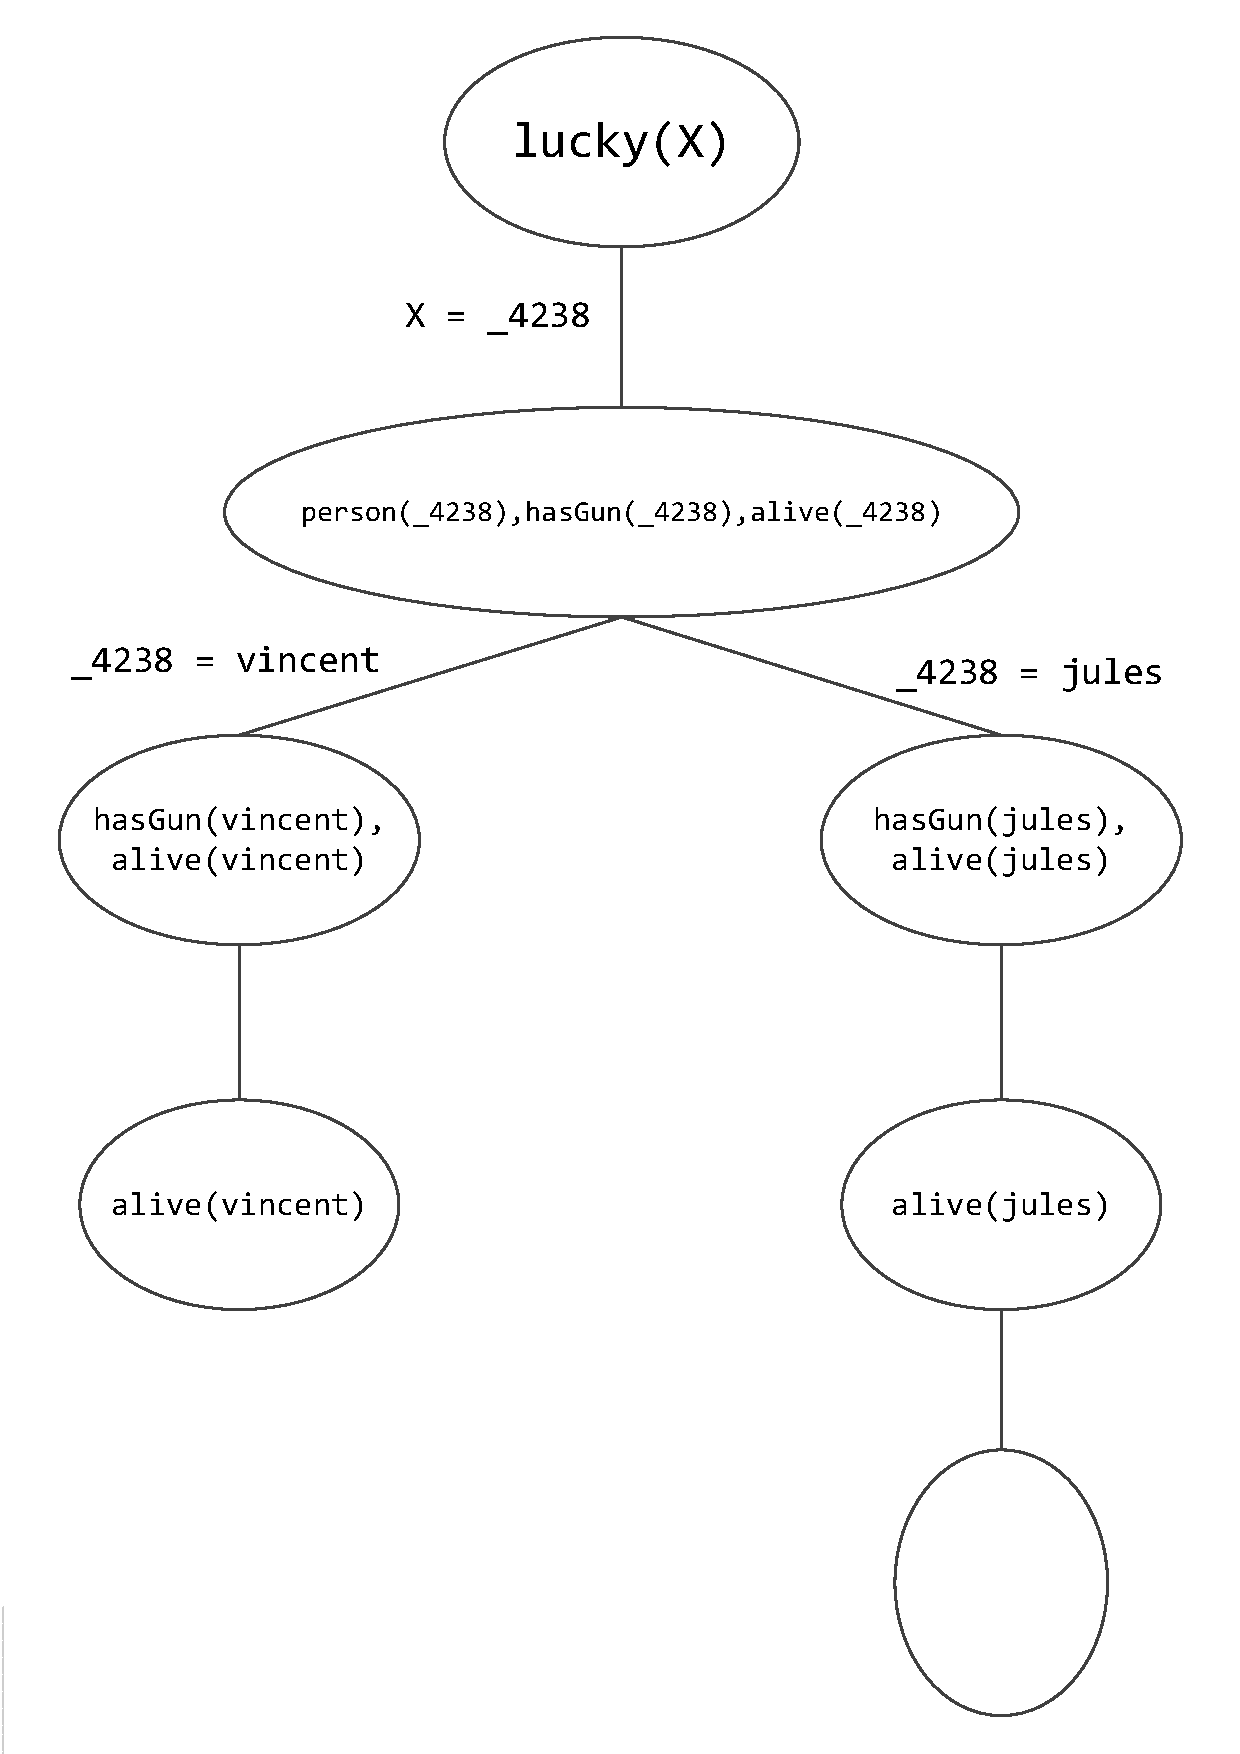
\includegraphics[scale=0.25]{stree}
	\end{figure}
\end{frame}

\subsection{Упражнения}

\begin{frame}
	\frametitle{\insertsection}
	\framesubtitle{\insertsubsection}
	В каких из перечисленных пар термы унифицированы? Где необходимо запишите значения переменных, необходимые для унификации.
	\texttt{\begin{enumerate}
			\item bread = bread
			\item 'Bread' = bread
			\item 'bread' = bread
			\item Bread = bread
			\item хлеб = котлета
			\item food(bread) = bread
			\item food(bread) = Bread
			\item food(Bread) = food(bread)
			\item food(хлеб,X) = food(Y,котлета)
			\item food(сухарики,X,пиво) = food(Y,чипсы,X)
			\item food(X) = X
			\item meal(food(bread),drink(beer)) = meal(food(X),Y)
			\item meal(food(bread),X) = meal(X,drink(beer))
	\end{enumerate}}
\end{frame}

\begin{frame}
	\frametitle{\insertsection}
	\framesubtitle{\insertsubsection}
	\textbf{Пусть дана следующая база знаний.}
	\texttt{\begin{itemize}
			\item[] witch(gullveig).
			\item[] god(freyja).
			\item[] god(odin).
			\item[] god('Vidarr').
			\item[] magic(X) :- witch(X).
			\item[] magic(X) :- wizard(X).
			\item[] magic(X) :- god(X).
	\end{itemize}}
	\textbf{Каким из запросов она удовлетворяет?}
	\texttt{\begin{enumerate}
			\item magic(witch).
			\item wizard(odin).
			\item magic('Vidarr').
			\item magic(Vidarr).
	\end{enumerate}}
\end{frame}

\begin{frame}
	\frametitle{\insertsection}
	\framesubtitle{\insertsubsection}
	\textbf{Дан следующий лексикон.}
	\texttt{\begin{itemize}
			\item[] word(article,a).
			\item[] word(article,every).
			\item[] word(noun,criminal).
			\item[] word(noun,'big kahuna burger').
			\item[] word(verb,eats).
			\item[] word(verb,likes).
			\item[] sentence(W1,W2,W3,W4,W5) :- word(article,W1), word(noun,W2), word(verb,W3), word(article,W4), word(noun,W5).
	\end{itemize}}
	Написать такой запрос, чтобы в результате получить список всех возможных фраз данного лексикона. Построить дерево поиска решений для одной из построенных фраз.
\end{frame}

\begin{frame}
	\frametitle{\insertsection}
	\framesubtitle{\insertsubsection}
	Имеется 6 слов: \textit{abalone, abandon, anagram, connect, elegant, enhance}, представленных в базе знаний следующим образом:
	
	
	\texttt{\begin{itemize}
			\item[] word(abalone,a,b,a,l,o,n,e).
			\item[] word(abandon,a,b,a,n,d,o,n).
			\item[] word(enhance,e,n,h,a,n,c,e).
			\item[] word(anagram,a,n,a,g,r,a,m).
			\item[] word(connect,c,o,n,n,e,c,t).
			\item[] word(elegant,e,l,e,g,a,n,t).
	\end{itemize}}
\end{frame}

\begin{frame}
	\frametitle{\insertsection}
	\framesubtitle{\insertsubsection}
	Реализовать предикат \texttt{crosswd/6 = crosswd(V1,V2,V3,H1,H2,H3)}, который бы заполнял данными словами следующий кроссворд таким образом, чтобы
	слова, идущие вертикально были первыми тремя аргументами, а слова, идущие горизонтально~--- последними тремя.
	\begin{figure}
		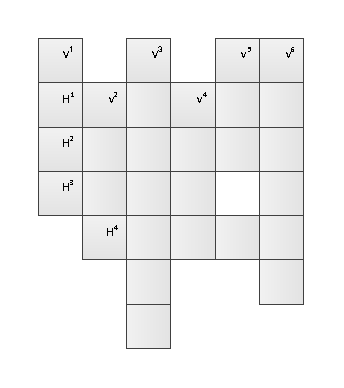
\includegraphics[scale=0.9]{crosswd}
	\end{figure}
\end{frame}